\chapter{Results}
\label{Chap:Results}

Our proposal for this thesis was to create an all day wrist motion activity monitor
that was small, cost effective and comfortable.
This device would also have to be able to record data for an entire day of activity,
decided as 16 hours.
The final device we have created can be worn on the wrist like a watch by using its strap.
Figure \ref{Fig:WristPhoto} shows a photograph of this arrangement when the device is worn around a wrist.
In this chapter we consider how we have compared against the requirements for the wrist activity monitor that we had set.
Users are expected to wear the device at the start of the day,
and press a button to start recording wrist motion movement data.
At the end of the day,
this device can be connected to a computer though a USB port and the data that has been logged can be transferred.
This data can then be analyzed or processed on the computer as needed.
We use WristView, a modified version of a software previously created by our group to visually display the data logged by our device. 
\begin{figure}
\begin{center}
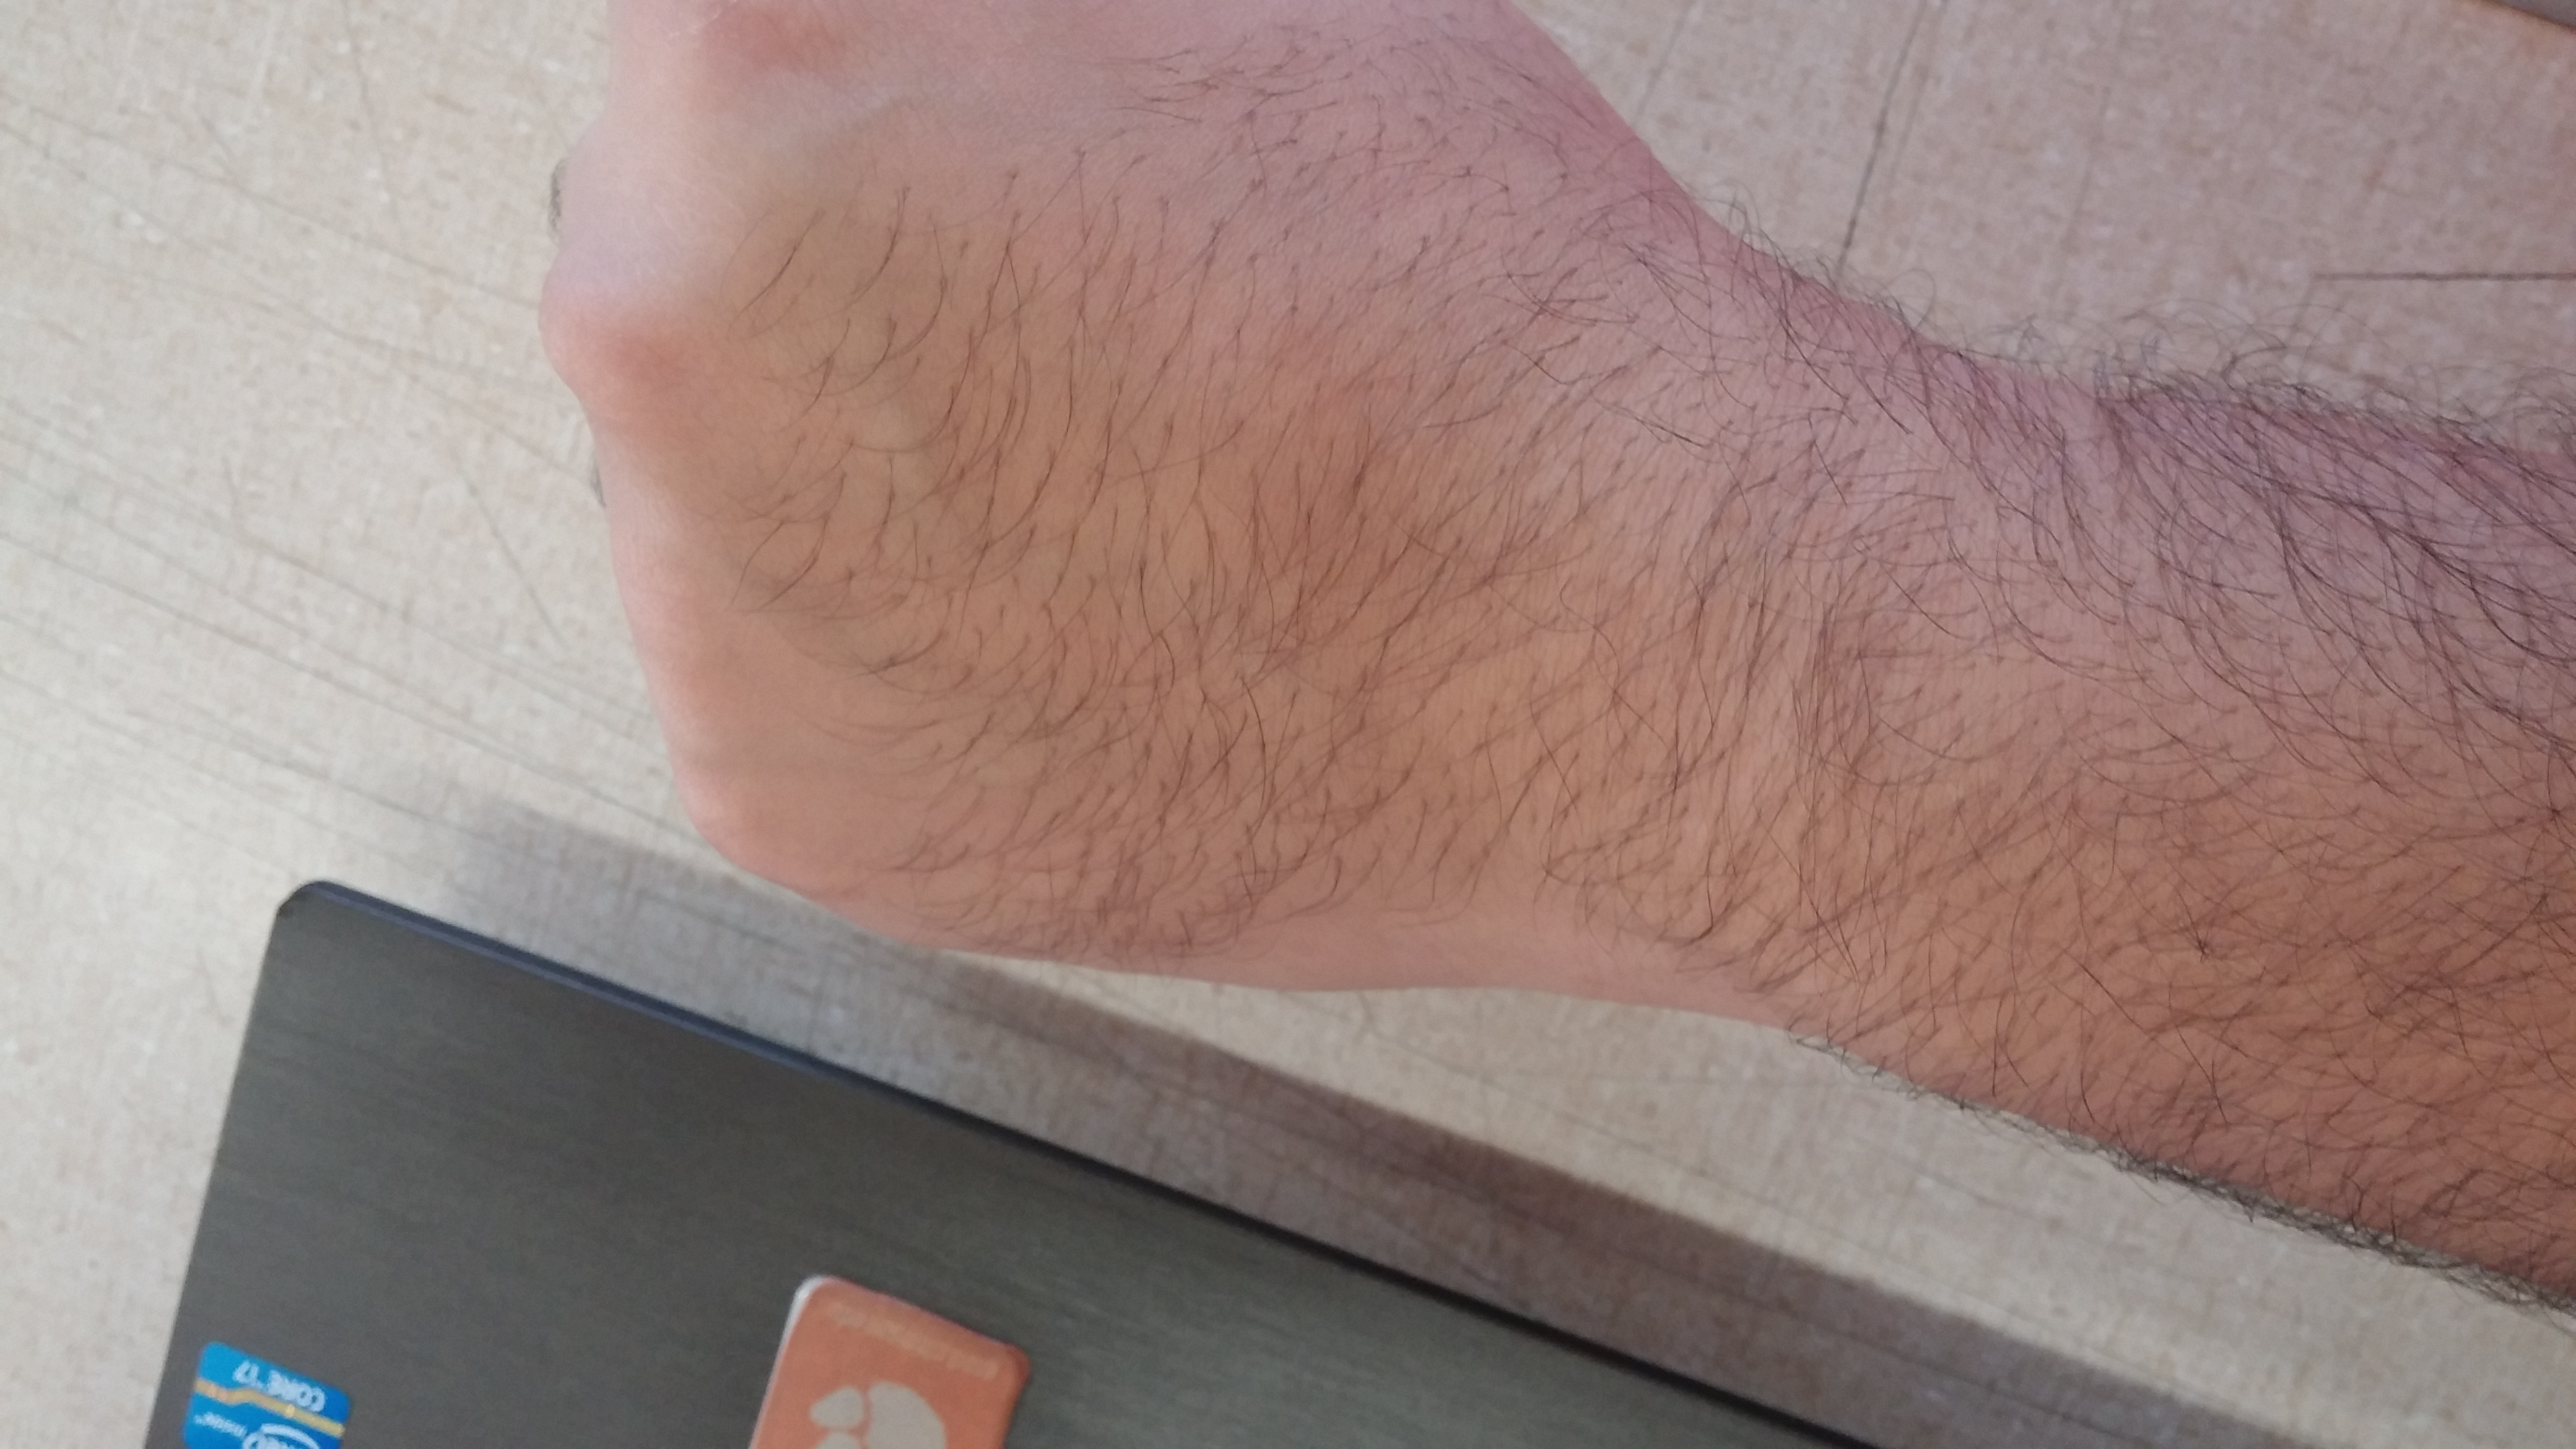
\includegraphics[width=\textwidth]{images/WristPhoto.jpg}
\caption{Photograph of the our activity monitor mounted on a wrist.}
\label{Fig:WristPhoto}
\end{center}
\end{figure}

\section{Size and comfort}
\label{Sec:ResultsSize}
The final PCB and components fit comfortably inside an OKW Ergo Minitec Small enclosure.
The dimensions of the device are the same as the enclosure,
52 mm X 32 mm X 15 mm.
A strap that is 12 mm wide and 20 cm long allows the user to wear this device on their wrist.
The device weighs 26.6g, including the strap.
The device was tested by two volunteers for 10 hours each,
and reported to be similar to a wrist watch with regards to comfort.
Note that this size is limited to the fact that we used a case available off the shelf.
If a custom design process was used which would allow for a case to be molded,
the size could be halved,
or spread around like a strap.

\section{Battery life}
\label{Sec:ResultsBatteryLife}
We needed to check if the battery life of the device met our specifications.
Battery manufacturers are known to inflate the battery life on data sheets for their products.
Current draw and how the battery is used also changes the output capacity of the battery.
Section \ref{Chap:Prototype} describes the methods used to test our prototype,
and the techniques used to measure the battery life of the product.
After testing the battery three times,
we concluded that the 130mAh battery would log wrist motion data for at least 24 hours,
which was higher than the required battery life for our device,
16 hours.
On standby mode (where the device is not recording any data), the battery life was up to one week.
Figure \ref{Fig:BatteryGraph} shows how the battery voltage drops versus time when it is actively recording motion data.
Data is not shown once the voltage dropped lower than 2.8 V.
The device was programmed to stop operating and enter standby mode
once the voltage was lower then 2.8 V.
This was to avoid recording incorrect data or corrupting the memory chip once supply
voltage was near the minimum level for components on our circuit.

\begin{figure}
\begin{center}
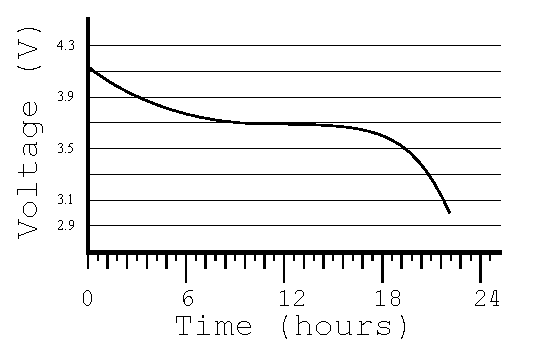
\includegraphics[width=0.7\textwidth]{images/BattLife.eps}
\caption{Graph showing battery life of the device.}
\label{Fig:BatteryGraph}
\end{center}
\end{figure}

\section{Software}
\label{Sec:ResultsSoftware}
We had been able to log data from the sensors into a memory chip,
and this data was then transferred to a computer in the form of a binary file.
Each byte in the file represents data recorded from a sensor,
with the time of the record being calculated by using the byte address.
Work done by our group previously could display motion data collected by an iPhone in a visual format.
We modified work done by Concha \cite{concha2014study} and created our own software to display the data logged by the wrist motion activity tracker.
This software, as mentioned in section \ref{Chap:Prototype},
was named WristView and allowed us to visually compare data captured by the device.
A screen shot of WristView can be seen in figure \ref{Fig:WristView}.
The figure shows the data plotted as amplitude versus time.
For acceleration data the amplitude was in g, where 1 g = 9.8 m/s$^2$. For gyroscopes, the data was in deg/sec.
Raw data from sensors usually contains noise.
WristView can smooth these signals based on code from PhoneView,
which uses an algorithm used by the research group previously \cite{concha2014study}.
This can be seen in figure \ref{Fig:WristViewSoomth}.
\begin{figure}
\begin{center}
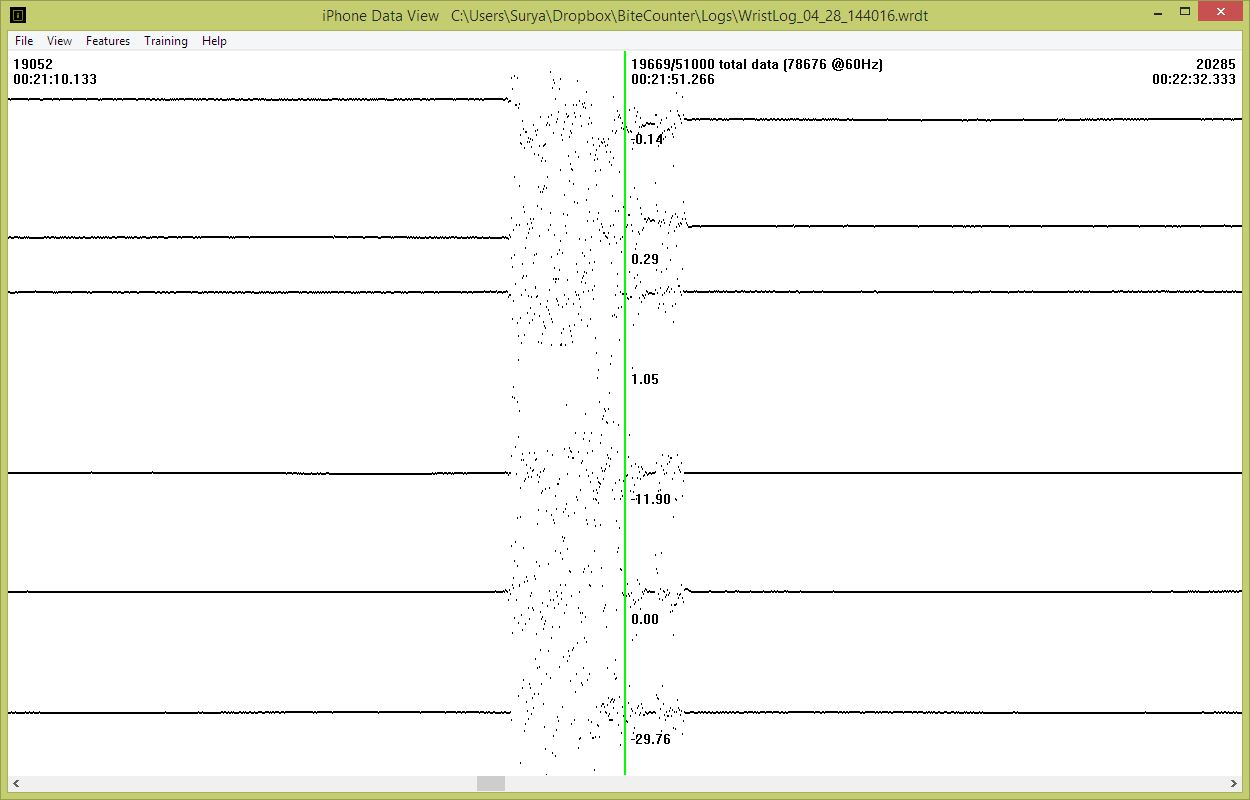
\includegraphics[width=0.7\textwidth]{images/WristView.jpg}
\caption{WristView displaying data captured by our prototype device. Top to bottom: Acceleration (X, Y, Z) and angular velocity (X, Y, Z)}
\label{Fig:WristView}
\end{center}
\end{figure}

\begin{figure}
\begin{center}
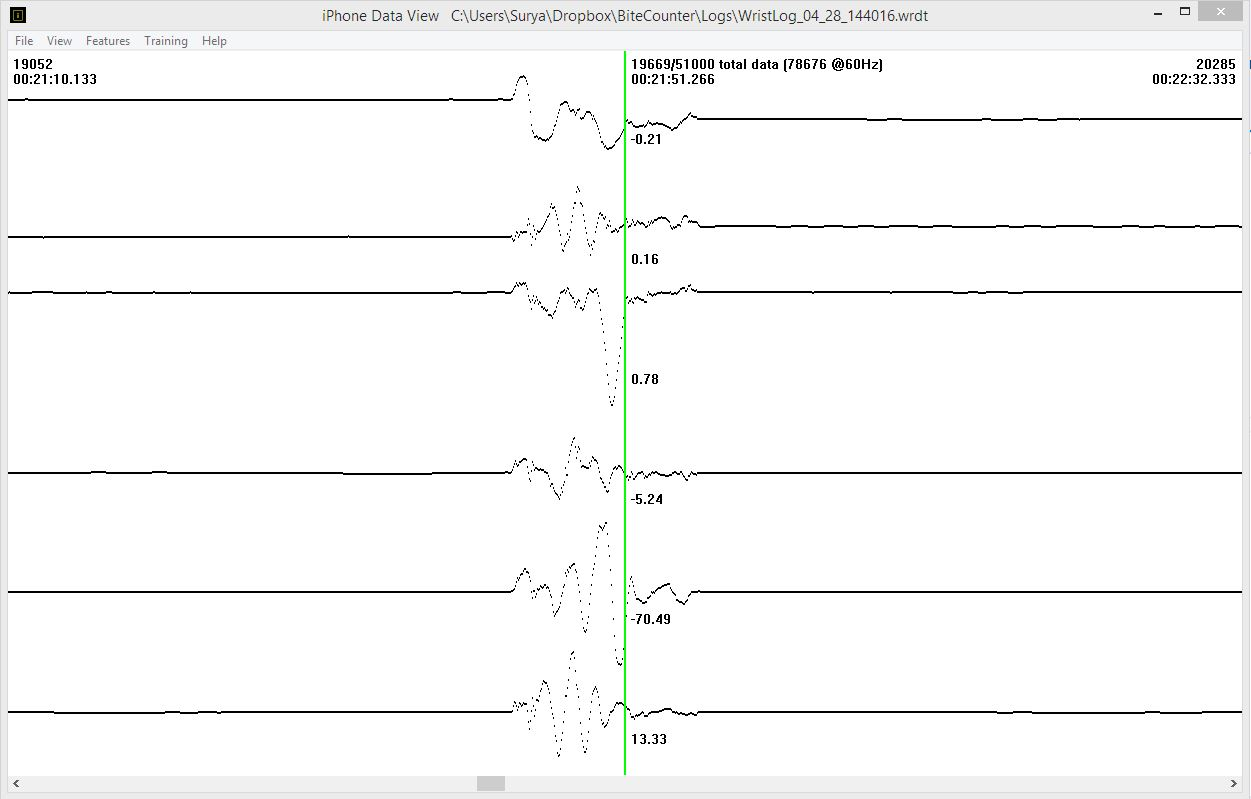
\includegraphics[width=0.7\textwidth]{images/WristSmooth.jpg}
\caption{WristView's smoothed data feature.}
\label{Fig:WristViewSoomth}
\end{center}
\end{figure}

\section{Device cost}
\label{Sec:DevCost}
Earlier, we had mentioned the different devices on the market marketed as research devices,
and also the high costs attached to using them.
The costs include expenditure on manufacturing and research.
After our device was created, 
we tabulated the cost of the parts of the device, and this can be seen in table \ref{BomTable}.
The total cost for the parts used per device was US\$52.5.
This number includes costs for PCB and stencil manufacture, but does not include any costs for the research of the device or hourly labor associated with assembly.
\inputfile{BOMTable.tex}

\inputfile{CompTable.tex}
\section{Comparison of devices}
\label{Sec:Comparison}
%Table \ref{Tab:DevCompare} shows that our device performs better than other devices on the market for our specific purpose, and that most devices lack the support for our bite counting application while maintaining comfort.
We see that our device cost is comparable to that of devices at the lower end of the spectrum.
Fitness Trackers like the Fitbit Zip cost \$49,
while research oriented devices like the SHIMMER cost \$249.
When procured in a large quantity so that wrist motion data can be captured
for 100 - 200 test subjects,
devices like the SHIMMER prove to be very expensive.
In comparison,
our work costs \$53 per device which allows us to obtain required quantities at lower costs.
Most Fitness trackers that are inexpensive, however,
do not allow custom programs or modifications.
Our work allows a high degree of modification and programmability compared to other
wrist mounted devices across the board.
Table \ref{Tab:DevCompare} shows only three devices which allow a significant level of programmability.
Since our device can be programmed using our custom code
it allows for a very high level of control.
Due to this, we can capture a higher resolution of wrist movement data
compared to other devices. Devices in table \ref{Tab:DevCompare} either do not offer this data at all,
offer it at a very low resolution (3 Hz for the Samsung Gear 2), or offer it for a short interval of time.

Devices that would suit our purpose, like the iPhone are not viable options due to their size or weight.
Our device measures 52 mm X 32 mm X 15 mm and weighs 26.6 g,
which makes it similar in size and weight to a watch.
This size gives the wearer a good level of comfort compared to wearing a heavy device like the iPhone on the wrist.
Most features of the device were obtained by limiting the components
to what we required for our purpose of tracking wrist movement data.
By not including components like a Bluetooth\texttrademark~module,
an LCD display or a speaker,
we have managed to keep the device small in size.
Note that this size was a limitation of the case we used,
an off the shelf option.
It is possible to reduce the size of the device much further by using industrial techniques and mass production methods to build a custom case.
The same philosophy of minimal components has allowed us to have an active battery life of 24 hours,
which is seen only in devices targeted towards research.
These facts show that for the application of logging wrist movement data for extended periods of time,
our customized device is the most economical option.

\section{Prototype challenges}
\label{Sec:ProtoChall}
Throughout this work we have emphasized the small sizes of the parts we used.
Integrating these parts into our device was a considerable challenge since we did not have access to industrial machines.
Before any of our parts could be connected and used,
they needed to be in a format that was easy to connect to.
The parts are manufactured to be used in an industrial setting,
and provided in surface mount packages.
An option available to us was to outsource the physical design of the device.
Once we had the design ready,
it could be provided to a manufacturer for soldering and assembling the device.
However this would at least double the cost of our device in the prototype phase, 
and not an acceptable solution.
Testing the different methods of soldering that could be used and then finally using
the solder reflow method as explained in section \ref{Chap:Prototype}
took a considerable amount of time.

Another issue we faced was devices overheating due to incorrect connection or a short circuit
created during the soldering phase.
To replace the burnt integrated chip,
we had to cut off the burnt chip from the PCB using an Exacto knife,
and then desolder the pins. This was done under a microscope.

Our first prototype had the device reporting incorrect motion data.
This was due to the fact that the SPI lines were extended beyond the typical specifications ($\approx$150 mm),
and the signal's power would drop rapidly as it traveled.
We accommodated for this in our PCB based prototype,
where the signal traveled very short distances ($\approx$5 mm).

\chapter{Conclusion and Future Work}
\label{Chap:Concl}
In this thesis, we proposed to create a device that would record data on 
the movement of a human wrist during a day.
This was motivated by the fact that wrist motion information can be used to count the number of bites
taken by a user,
or predict the tool being used to take a bite.
Other devices in the market did not have the required sensors to track this motion,
or had extra features which increased the size of the device and reduced its battery life.
As mentioned in Chapter \ref{Chap:Results},
we were able to create a wrist motion activity tracker that records this data at a good resolution,
allows a high level of customization,
has a sufficient battery life and has a size that is comfortable to wear for extended periods of time.

Future work for the device
involves the addition of a time synchronization feature when the device is connected to a computer.
This would store the local time of the user on the wrist motion activity tracker,
and will allow the device to time stamp when it was stopped and started,
allowing data analysis to be performed to detect periods of eating and non-eating.

In our wrist motion activity tracker,
a large amount of power is utilized by the sensors which are always turned on.
While we were working through this thesis,
newer technology has allowed sensor manufacturers to improve the sensors they are producing.
Some new sensors now come with microcontrollers in-built which can be programmed by the user.
In our work,
the sensors we used
were operating based on an internal clock of 8 KHz.
We would then read from the sensors at 15 Hz.
Since we only need the sensors to be polled at 15 Hz,
it should be possible to decrease the rate at which the sensors are operating.
If the sensors could sleep between two readings,
it would allow us to have a huge improvement in battery life as it would reduce the average current draw by the sensors.

When we compared the different devices on the market,
we noticed that the wrist band device MYO uses EMG sensors coupled with accelerometer and gyroscope data to increase the accuracy of detection.
Thalmic Labs \cite{Web:GetMyo} claims that the EMG sensors help estimate the pose of a users hand with very high accuracy.
We consider that this claim might be true,
and we plan to incorporate these newer EMG sensors that are smaller in future work.

Creating a dataset of wrist motion data using this device is our next step forward.
We plan to have 100 - 200 subjects wear the device for up to
2 weeks each to record their wrist movement data.
This may require the production of 20 - 50 units of the device.
This large data set will be used to improve the algorithms for detecting eating events and counting the bites during these events.